\clearpage
% \subsection{\label{Run14TPC_YF}Run11 TPC analysis YF}

\newcommand{\ttbs}{\char'134}
% \newcommand{\AmS}{{\protect\the\textfont2A\kern-.1667em\lower.5ex\hbox{M}\kern-.125emS}}
\hyphenation{author another created financial paper re-commend-ed}
\newcommand{\pt}{$p_{T}$ }
\newcommand{ \bfg }{\begin{figure}[]}
\newcommand{ \efg }{\end{figure}}
\newcommand{\dzero}{$D^{0}$ }



%%%%%%%%%%%%%%%%%%%%%%%%%%%%%%%%%%%%%%%%%%%%%%%%%%
%                                                %
%    BEGINNING OF TEXT                           %
%                                                %
%%%%%%%%%%%%%%%%%%%%%%%%%%%%%%%%%%%%%%%%%%%%%%%%%%

Since at \pt\ $<$ 2 GeV/$c$ a discrepancy was found between new data from Run14 with HFT and published data from Run10+Run11. A re-analysis on Run11 data was performed to check if anything was incorrect. The analysis cuts are the same as in previous analysis note:

https://drupal.star.bnl.gov/STAR/system/ \\

files/dzeroAuAu$\_$updated.pdf, also listed in Xiaolong 's analysis, see next section. The only difference is varying DCA cut with $<$ 1 cm or $<$ 2 cm.

The raw signals as a function of \pt\ from part of Run11 data with 85\% of full statistics were extracted as Fig.\ref{D0inpt1},

\bfg \centering
%\vspace{-0.2in}
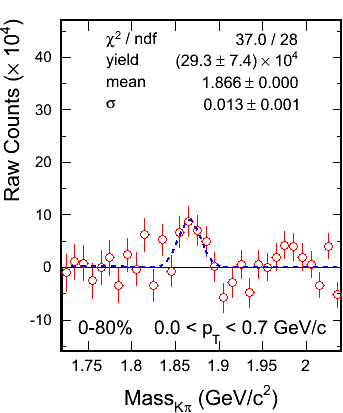
\includegraphics[width=0.3\textwidth]{figure/Run11_YF/D0_0-80_1_7_signal.png}
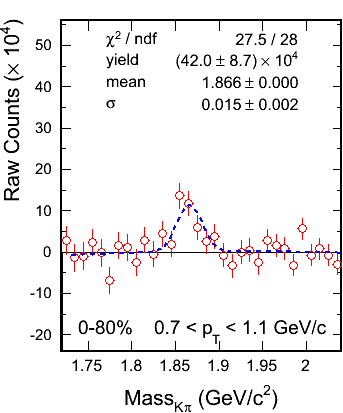
\includegraphics[width=0.3\textwidth]{figure/Run11_YF/D0_0-80_8_11_signal.png}
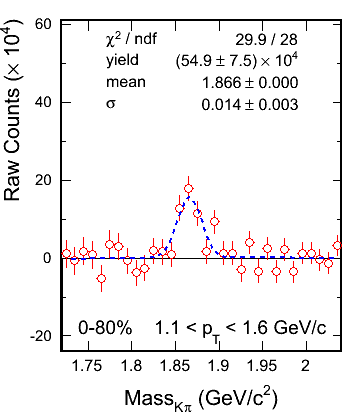
\includegraphics[width=0.3\textwidth]{figure/Run11_YF/D0_0-80_12_16_signal.png}
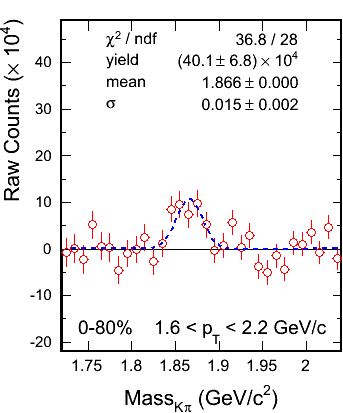
\includegraphics[width=0.3\textwidth]{figure/Run11_YF/D0_0-80_17_22_signal.png}
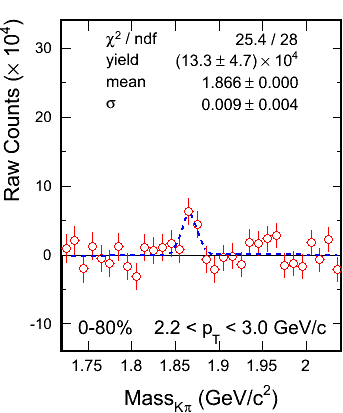
\includegraphics[width=0.3\textwidth]{figure/Run11_YF/D0_0-80_23_30_signal.png}
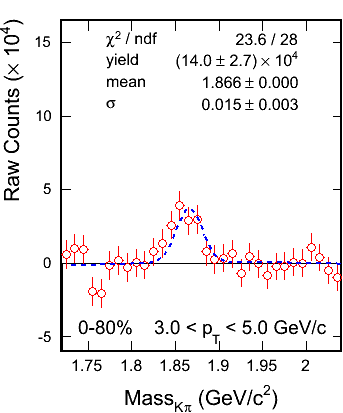
\includegraphics[width=0.3\textwidth]{figure/Run11_YF/D0_0-80_31_50_signal.png}
%\vspace{+0.2in}
\caption{\pt\ dependence of \dzero\ signals in 0-80\% from partial Run11 data.}
\label{D0inpt1}
\efg

The raw signals were compared with Xiaolong 's independent analysis and found to be consistent, shown in Fig.\ref{rawsig}. The slight lower yield in Xiaolong 's analysis is due to the tight DCA cut $<$ 1 cm, while the DCA cut applied here is $<$ 2 cm.

\bfg \centering
%\vspace{-0.2in}
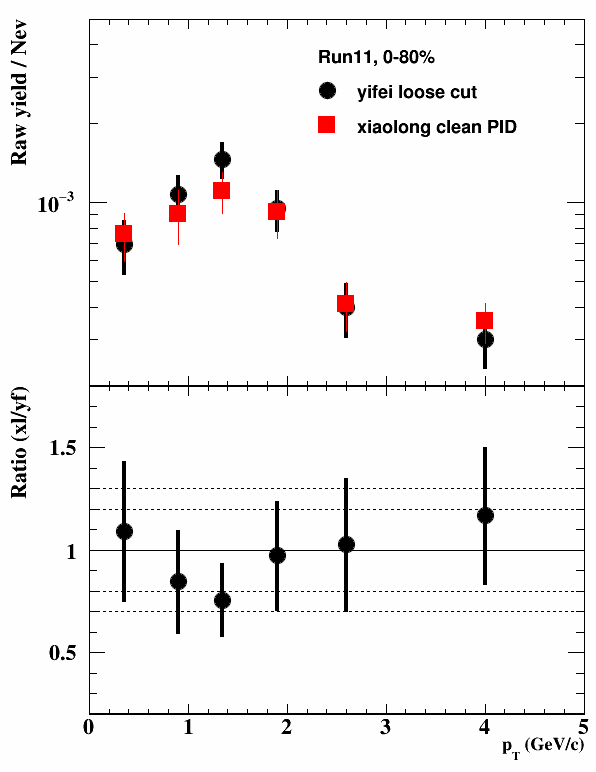
\includegraphics[width=0.6\textwidth]{figure/Run11_YF/RawY_0_80.png}
\caption{Raw signals comparison with Xiaolong 's.}
\label{rawsig}
\efg

In early days, there was no vertex detector, we had to use random combination of decay products to reconstruct \dzero\ meson in hadronic channel, which suffered from huge combinatorial background. The way to improve the significance was to enrich the kaon and pion PID probability and enhance the statistics as much as possible at the same time. Thus we developed a hybrid method: at low \pt\ we used TOF PID to ensure the purity of kaons and pions, at high \pt , if there was an available TOF matching, we applied TOF PID, otherwise we used TPC PID to enhance the PID efficiency. But an issue was found in the code, that the condition to reject those tracks without matching to TOF at low \pt\ was different from what we used to calculate the efficiency. In data analysis, we reject those tracks with no TOF matching, while in calculating efficiency we reject those tracks with no TOF matching and those with no valid $\beta$ information in TOF. This introduces about 15\% difference at low \pt\ but does not affect high \pt much. 

\bfg \centering
%\vspace{-0.2in}
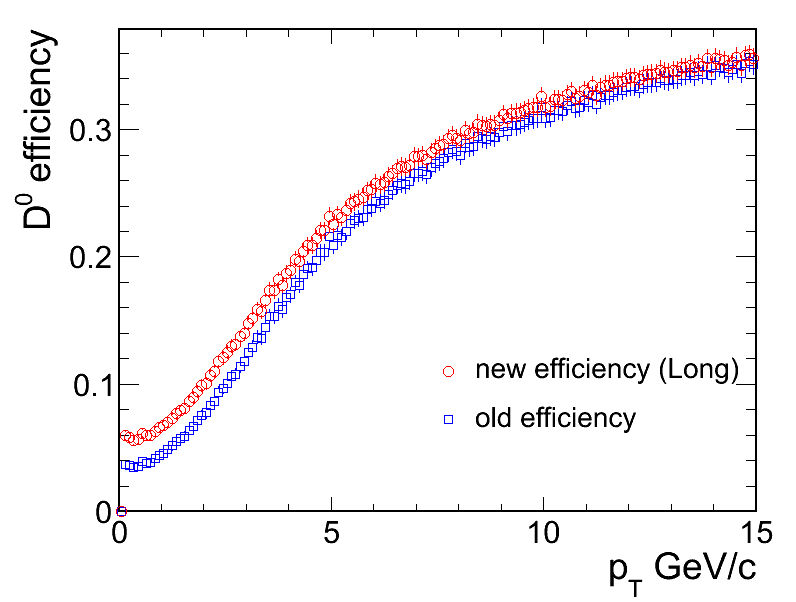
\includegraphics[width=0.6\textwidth]{figure/Run11_YF/eff.png}
\caption{New efficiency checked from Long compared with old one.}
\label{effnew}
\efg

The other issue is that we applied an additional $DCA_{XY}$ cut efficiency in previous analysis. This cut was used in TOF matching algorithm (in TOFMatchMaker) to require tracks with a distance of closest approach to the beam line in xy plane within 1 cm. This efficiency was studied in early days and found there was about up to 20\% of tracks at low \pt\ rejected with this cut, see Fig.\ref{DCAxyeff}. However, when we studied TOF matching efficiency, we used a data driven method and this efficiency should be already included. Thus we double counting this efficiency.

\bfg \centering
%\vspace{-0.2in}
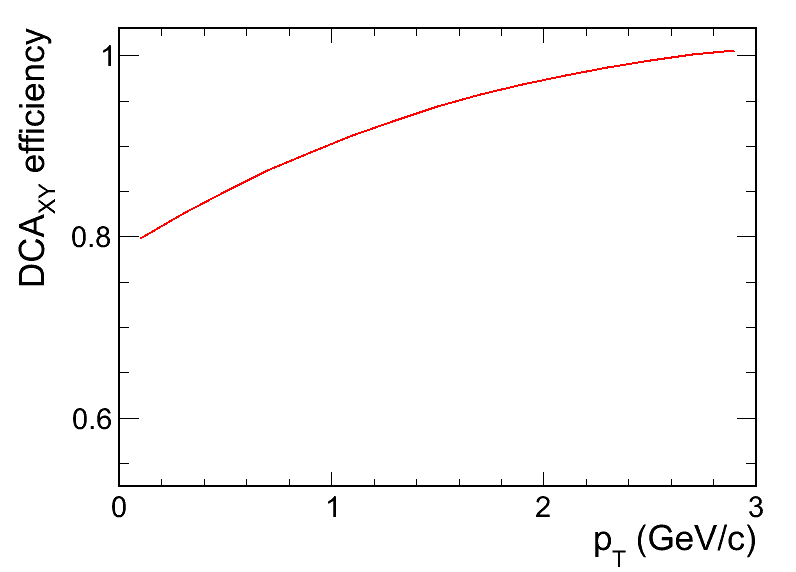
\includegraphics[width=0.6\textwidth]{figure/Run11_YF/DCAxyEff.png}
\caption{$DCA_{XY}$ efficiency.}
\label{DCAxyeff}
\efg

Long checked correction with new efficiencies ...


%%%%%%%%%%%%%%%%%%%%%%
% End of tex  %
%%%%%%%%%%%%%%%%%%%%%%

